\documentclass[journal]{IEEEtran}
\usepackage[T1]{fontenc}
\usepackage{amsmath,amssymb}
\usepackage{graphicx}
\usepackage{booktabs}
\usepackage{multirow}
\usepackage{algorithm}
\usepackage{algpseudocode}
\usepackage{xcolor}
\usepackage{xurl}
\usepackage[hidelinks]{hyperref}

\newcommand{\sg}{\operatorname{sg}}
\newcommand{\pp}{\,pts}

\begin{document}

\title{Protocol-Faithful Dataset Distillation for Few-Step Fine-Tuning: Lessons from the MVEO 2026 Data-Centric Land Cover Challenge}

% TODO: check the name order, add co-authors, affiliations and e-mail addresses.
\author{Uriel~Nguefack%
\thanks{Affiliation and contact details to be added.}}

\markboth{Draft, \today}{Nguefack: Protocol-Faithful Dataset Distillation for Few-Step Fine-Tuning}

\maketitle

\begin{abstract}
In the MVEO 2026 Data-Centric Land Cover Classification Challenge, the model and the training code are fixed and
participants only choose the training images. An ImageNet ViT-B/16 is fine-tuned on them for five epochs with
AdamW, and the score rewards both accuracy on EuroSAT and a small number of images. We first show that this recipe
makes training very short: a set of $n$ images gives only $5\lceil n/32\rceil$ optimizer steps, the first Adam
steps move every weight by almost the same amount, and the new classifier head hardly moves. We then distill
training sets by optimizing the pixels of real images through an exact simulation of the official training run,
with all its steps unrolled. A checkpointed backward pass keeps memory at 12.4~GB for 20 steps of ViT-B/16, and a
smoothed Adam step carries useful gradients through sign-like updates. We also show that the usual cross-entropy
outer loss mostly rewards confident logits, and we replace it with the cross-entropy at the best-fitting
temperature. With 120 images, validation accuracy of the official script goes from 87.2\% for k-means medoids to
89.9\%, averaged over six seeds, while the images change by 0.26 gray levels on average. Finally, we study what
happens when the images are fitted to the one run that the official script makes with its default seed: ten
images then reach 80.6\% on that run and the first place of the leaderboard, but only 52\% on other seeds. Single-run
evaluation lets a distilled set fit the evaluation run itself, so we suggest that such challenges average over
several seeds. Code and all submitted images are released.
\end{abstract}

\begin{IEEEkeywords}
Dataset distillation, data-centric learning, vision transformers, land cover classification, EuroSAT, fine-tuning.
\end{IEEEkeywords}

\section{Introduction}

\IEEEPARstart{L}{abeled} data is the expensive part of most remote sensing projects. A large body of work therefore
asks how much of a training set is really needed, and dataset distillation pushes this question to its limit: it
replaces a full training set with a few synthetic images that, once used for training, give a model close to the one
trained on all the data~\cite{wang2018dd,zhao2021dc,cazenavette2022mtt}. Most of this work trains small networks from
scratch for hundreds or thousands of steps. Practice in Earth observation looks different. People start from a large
pre-trained model and fine-tune it briefly on a small labeled set.

The Data-Centric Land Cover Classification Challenge of the MVEO 2026 workshop~\cite{mveo2026} puts this setting
into a clean form. The model (ViT-B/16 pre-trained on ImageNet~\cite{dosovitskiy2021vit}) and the training script
are fixed. Participants submit a set of labeled $64\times64$ RGB images, the organizers fine-tune the model on them
with the official script, and the predictions on a hidden EuroSAT~\cite{helber2019eurosat} test set give the
accuracy. The score adds a term that falls with the number of images $n$, so ten good images can beat a few hundred
average ones.

This paper describes what we learned while building our entries. Our first finding is that the fixed recipe is far
from the usual distillation setting. A set of $n$ images gives only $5\lceil n/32\rceil$ AdamW steps: 5 steps for
10 images, 20 steps for 120. In so few steps Adam behaves like sign descent~\cite{balles2018dissecting,kunstner2023sign},
so the content of the images mostly decides the sign of each weight update, not its size. The new classifier head
starts at random and barely moves, so the backbone has to bring each class onto a random direction. Real images
are not the best training signal in this regime. With 1024 real images per step the model reaches 60.4\% after 5
steps, while the best network that 5 steps can reach is above 78.8\%.

Our second finding is that distillation works here if it follows the protocol exactly. We call our method
protocol-faithful distillation (PFD). It simulates the official run step by step: the same shuffling and batch
sizes, the same random crops and flips, the same AdamW update and learning-rate schedule. It then back-propagates
from the loss on real training images, through all the training steps, to the pixels. Three parts make this
practical. A checkpointed reverse pass rebuilds one training step at a time, so memory does not grow with the
number of steps. A smoothed Adam step in the backward pass gives useful gradients through updates that are almost
pure signs. And a scale-free outer loss stops the optimization from spending its effort on confident logits.

Our third finding is about evaluation. The official script fixes the random seed, so the whole training run (head
initialization, shuffling, crops) is the same every time it is executed. We recorded that run and fitted ten images
to it. They reach 80.6\% validation accuracy on it and the first place of the public leaderboard, while the same
images reach only 52\% on average with five other seeds. The 120-image sets built for all seeds behave the same on
every seed. We report both kinds of results and keep them apart in every table.

Our contributions are:
\begin{itemize}
\item an analysis of the few-step fine-tuning regime of the challenge: the step staircase, the sign-like Adam
updates, the frozen head, and the gap between the real-data oracle and what a few steps can reach;
\item PFD, a distillation method that unrolls the full official training of ViT-B/16 with constant memory, with a
smoothed Adam backward pass and a scale-free outer loss;
\item a careful evaluation with the official script over several seeds, including a list of ideas that did not help;
\item a measurement of how much a distilled set can gain by fitting a single evaluation run, with simple
recommendations for future challenges.
\end{itemize}
The code, the logs of every run and the exact images of all our submissions are available in our
repository.\footnote{\url{https://github.com/nguefackuriel/Land-Cover-Classification-Kaggle-MVEO} (to be made public after the challenge).}

\section{Related Work}

\subsection{Dataset distillation}
Wang \emph{et al.}~\cite{wang2018dd} learned synthetic images by back-propagating through a few training steps of a
small network. Later methods replaced this costly bilevel problem with cheaper surrogates: matching the gradients
of real and synthetic batches~\cite{zhao2021dc}, with differentiable augmentation~\cite{zhao2021dsa}; matching
feature distributions~\cite{zhao2023dm}; or matching segments of expert training
trajectories~\cite{cazenavette2022mtt,guo2024datm}. At ImageNet scale, recent methods recover images from a trained
model and train the student on soft labels~\cite{yin2023sre2l,sun2024rded}. Qin \emph{et al.}~\cite{qin2024label}
showed that much of the gain of these methods comes from the soft labels themselves. The challenge allows only hard
labels and a fixed recipe, which brings the problem back to its original form: images that are good for one given
training procedure. The winners of the ECCV 2024 distillation challenge made a similar observation and removed soft
labels to match the official evaluation~\cite{zhou2024mdatm}. The inner training loop has also been studied
directly. Li \emph{et al.}~\cite{li2025atbptt} truncate back-propagation through time adaptively. DD-Ranking~\cite{li2025ddranking}
shows that evaluation details can change the ranking of methods.

\subsection{Pre-trained models and remote sensing}
Cazenavette \emph{et al.}~\cite{cazenavette2025lgm} distill images for linear probes trained on frozen
self-supervised features. In our case the whole backbone is fine-tuned, which changes the problem: the features move,
and the update of every weight is decided by the images. In remote sensing, Xu \emph{et al.}~\cite{xu2026dpd}
generate realistic distilled sets with a diffusion model guided by class prototypes, for convolutional networks
trained from scratch. We are not aware of distillation work that targets the full fine-tuning of a pre-trained
vision transformer in a few optimizer steps.

\subsection{Differentiating through training}
Back-propagating through a training run goes back to work on hyperparameter
optimization~\cite{maclaurin2015reversible}. Memory is the main obstacle. We use checkpointing~\cite{chen2016checkpoint}
at the level of whole optimizer steps. To pass gradients through Adam's sign-like steps we use a straight-through
estimator~\cite{bengio2013ste}: the forward pass is exact and the backward pass uses a smoothed version.

\subsection{Small changes that steer training}
Small pixel changes can flip the prediction of a trained network~\cite{szegedy2014intriguing,goodfellow2015explaining}.
They can also act at training time: error-minimizing noise makes data useless for training~\cite{huang2021unlearnable}.
Our distilled images are an example of the opposite effect, invisible changes that make the training images more
useful. Like robust adversarial examples~\cite{athalye2018eot}, they are optimized in expectation over the random
transformations they will meet.

\subsection{Seeds and leaderboards}
Results in deep learning change with the random seed~\cite{bouthillier2021variance,picard2021seed}, and repeated
submissions can overfit a public leaderboard~\cite{blum2015ladder}. The challenge evaluates one run with a fixed seed.
Section~\ref{sec:seed42} measures how much a training set can gain from that single run.

\section{The Challenge Protocol}
\label{sec:protocol}

\subsection{Data and score}
The data comes from EuroSAT RGB~\cite{helber2019eurosat}: $64\times64$ Sentinel-2 image patches in ten land cover
classes. The challenge provides 18\,900 training, 4\,050 validation and 4\,050 test images. The labels are anonymous
(\texttt{class\_00} to \texttt{class\_09}), but the images show that they follow the usual alphabetical order of
the EuroSAT classes, which we use in the figures. A submission lists $n$ training images and the test predictions of
the model trained on them. The score is
\begin{equation}
S = \tfrac{1}{2}\,a + \tfrac{1}{2}\left(1 - \frac{\ln n}{\ln 18900}\right),
\label{eq:score}
\end{equation}
where $a$ is the test accuracy. Each halving of $n$ adds 0.035 to the score, the same as 7 points of accuracy.
Fig.~\ref{fig:landscape} shows the lines of equal score.

\subsection{Training recipe}
The official script \texttt{baseline.py} loads ViT-B/16 with its ImageNet weights and replaces the last layer with
a new linear layer of 10 outputs, initialized at random by PyTorch. It trains all weights with AdamW~\cite{loshchilov2019adamw}
(learning rate $3\times10^{-5}$, weight decay 0.05, batch size 32) for five epochs. The learning rate follows a
cosine schedule that is updated once per epoch, so the five epochs use $3.0$, $2.7$, $2.0$, $1.0$ and
$0.3\times10^{-5}$. The data loader shuffles the images at each epoch and keeps the last, smaller batch. Training
images go through a random resized crop (75\% to 100\% of the area, output $224\times224$) and random horizontal and
vertical flips. Validation and test images are resized to $256\times256$ and center-cropped to $224\times224$.
The script keeps the epoch with the best validation accuracy and predicts the test set with it. Its defaults are
seed 42 and two data-loading workers. With these defaults the run is deterministic: on our A100 GPU three runs on
the same images gave identical predictions.

\begin{figure}[t]
\centering
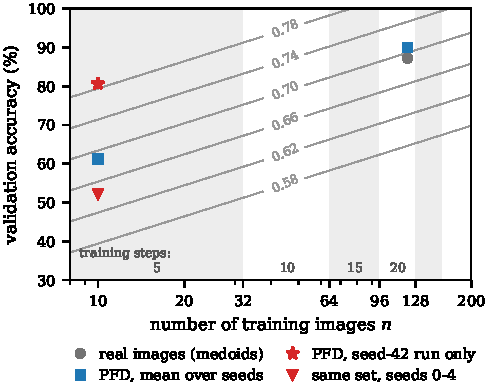
\includegraphics[width=\columnwidth]{figures/score_landscape.pdf}
\caption{Lines of equal score (\ref{eq:score}) as a function of the number of images $n$ and of the accuracy. Gray
bands show the number of training steps $5\lceil n/32\rceil$. Points are official validation accuracies of our
sets: the mean over seeds for sets built for all seeds, and the seed-42 run alone for the set fitted to that run.}
\label{fig:landscape}
\end{figure}

\subsection{What the recipe implies}

\begin{table}[t]
\centering
\caption{Training steps and size term of the score for some set sizes.}
\label{tab:steps}
\begin{tabular}{rcccc}
\toprule
$n$ & batches per epoch & last batch & steps $K$ & size term \\
\midrule
10 & 1 & 10 & 5 & 0.383 \\
20 & 1 & 20 & 5 & 0.348 \\
32 & 1 & 32 & 5 & 0.324 \\
33 & 2 & 1 & 10 & 0.322 \\
64 & 2 & 32 & 10 & 0.289 \\
96 & 3 & 32 & 15 & 0.268 \\
97 & 4 & 1 & 20 & 0.268 \\
112 & 4 & 16 & 20 & 0.260 \\
120 & 4 & 24 & 20 & 0.257 \\
128 & 4 & 32 & 20 & 0.254 \\
\bottomrule
\end{tabular}
\end{table}

\emph{Few steps.} Table~\ref{tab:steps} lists the number of optimizer steps $K = 5\lceil n/32\rceil$. Going from 32
to 33 images doubles the number of steps, but the 33rd image forms a batch of one at the end of each epoch.

\emph{Sign-like updates.} With Adam~\cite{kingma2015adam}, the update of a weight is
$\eta_t\,\hat m_t/(\sqrt{\hat v_t}+\epsilon)$, where $\hat m_t$ and $\hat v_t$ are bias-corrected running means of the
gradient and of its square. At the first step $\hat m_1/\sqrt{\hat v_1} = g_1/|g_1|$, so every weight moves by
exactly $\pm\eta_1$, whatever the size of its gradient. The next steps stay close to sign descent with
momentum~\cite{balles2018dissecting,bernstein2018signsgd}. The images therefore choose the direction of each weight
update, not its size, and a batch of one image moves the network as far as a batch of 32.

\emph{A frozen head.} The new head starts with weights of order $1/\sqrt{768}\approx0.036$. Adam moves each weight
by roughly the learning rate per step at most, so after 20 steps a head weight has moved by at most about
$3.6\times10^{-4}$, around 1\% of its initial size. The head stays almost random, and the backbone does the learning: it has to move
the features of each class towards a random direction that changes with the seed. A good training set must
therefore work for any head.

\emph{Real data is not the ceiling.} We trained with the official recipe but computed each step on 1024 fresh real
images instead of 32. This ``oracle'' reaches 60.4\%, 80.1\% and 91.7\% after 5, 10 and 20 steps (seed 42).
We also searched directly for the best network that the recipe can reach: every weight can move by at most about the sum
of the learning rates ($9\times10^{-5}$ for 5 steps), so we ran projected sign descent on the training loss inside
this box. It found networks with 78.8\% after 5 steps and 94.4\% after 10 steps. Few-step training is thus limited
by the direction of the updates, and well-chosen images can in principle beat the full training set.

\section{Protocol-Faithful Distillation}
\label{sec:method}

\subsection{Objective}
Let $x=(x_1,\dots,x_n)$ be the training images with fixed labels $y$. One official training run depends on $x$ and
on three random choices: the head initialization $h$, the shuffling $\pi$ and the augmentations $\alpha$. It ends with
weights $\theta_K(x;h,\pi,\alpha)$. We want images that give a good model on average over these choices:
\begin{equation}
\min_x\; \mathbb{E}_{h,\pi,\alpha}\Big[\,\ell\big(\theta_K(x;h,\pi,\alpha);\,\mathcal{R}\big)\Big],
\label{eq:objective}
\end{equation}
where $\ell$ is a loss on a batch $\mathcal{R}$ of 512 real training images, taken with the evaluation transform.
Validation images are never used in this loss. We only use them to choose checkpoints.

\subsection{Exact forward simulation}
We wrote a GPU copy of the official pipeline. It uses the same model code and initialization, the same batch
construction (shuffle, batches of 32, the smaller last batch kept), the same random resized crop and flips, the same
AdamW update and the same per-epoch schedule. The inner training runs in bfloat16. For our 120-image sets, our copy
gives a six-seed mean validation accuracy within 0.1 point of the official script (Section~\ref{sec:fidelity}).

\subsection{Checkpointed reverse pass}
The gradient of (\ref{eq:objective}) with respect to $x$ goes through all $K$ training steps. Each step contains a
forward and backward pass of ViT-B/16, and the graph of the training run grows quickly: six unrolled steps at $n=40$
already took 39.7~GB. During the forward pass we store only the weights and the Adam moments $(\theta_t, m_t, v_t)$ before each step,
along with the batch indices and the state of the random generator. During the reverse pass we rebuild the graph of
one step at a time from these states, propagate the adjoints of $(\theta_t, m_t, v_t)$ through it, and collect the
gradient with respect to the pixels. GPU memory then stays constant in $K$. At $n=120$ with $K=20$ the states take
21~GB. Kept on the GPU, the run needs 30~GB; kept in pinned CPU memory, it needs 12.4~GB of GPU memory and about
10~s per head on an A100.
On a short problem where the full graph fits in memory, the gradients of the two methods have a cosine similarity of
0.9998.

\subsection{A smoothed Adam step for the backward pass}
The derivative of a sign is zero almost everywhere, and early Adam steps are close to signs. We keep the exact Adam
step in the forward pass and use a smoothed step in the backward pass, in the style of a straight-through
estimator~\cite{bengio2013ste}:
\begin{equation}
\tilde u_t = \frac{\hat m_t}{\sqrt{\hat v_t + \tau^2\,\overline{\hat v_t} + \epsilon^2}},\qquad
u_t = \tilde u_t + \sg\!\big(\hat u_t - \tilde u_t\big),
\label{eq:ste}
\end{equation}
where $\hat u_t = \hat m_t/(\sqrt{\hat v_t}+\epsilon)$ is the exact step, $\overline{\hat v_t}$ is the mean of
$\hat v_t$ over each weight tensor, $\sg$ stops the gradient, and $\tau=0.3$. The value of $u_t$ is exact, and its
gradient is that of a step where very small gradients no longer get a full-size update.

\subsection{Randomness}
At each outer step we draw new heads from the same distribution as the official script, a new shuffling and new
crops and flips, and average the gradient over two such runs. Averaging over heads is important because the head
decides where each class must go (Section~\ref{sec:protocol}). Averaging over augmentations follows the expectation
over transformations of~\cite{athalye2018eot}.

\subsection{A scale-free outer loss}
With $\ell$ equal to the cross-entropy on real images, the outer loss fell by 30\% during optimization while
accuracy rose by only 2 points. After 20 steps the logits are small and badly calibrated: on our best images, the
temperature that minimizes the real loss is $T^\ast\approx0.32$, and dividing the logits by it lowers the loss from
0.63 to 0.26. Much of the plain cross-entropy is about the scale of the logits, which does not change any prediction.
We therefore fit the temperature on each real batch and use
\begin{equation}
\ell = \mathrm{CE}\big(z/T^\ast,\,y\big),\qquad T^\ast = \arg\min_{T}\,\mathrm{CE}(z/T,\,y),
\label{eq:scalefree}
\end{equation}
where $z$ are the logits of the trained network on $\mathcal{R}$. We search $T^\ast$ on a grid of 121 values between
0.01 and 10, without gradient. Since $T^\ast$ is a minimizer, its own variation does not change the gradient (the
envelope theorem). This loss only rewards a better ranking of the classes.

\subsection{Pixel updates and export}
We start from real images: k-means medoids in the ViT-B/16 feature space, the same number per class.
The pixels are kept in logit space, $x=\sigma(z)$, and updated with a step normalized by its largest entry,
$z \leftarrow z - \varepsilon_k\, g/\|g\|_\infty$, with $\varepsilon_k$ following a cosine schedule (from 0.05 to 0.01
for a fresh run). This moves only the pixels with the largest gradients, by small amounts. The submitted images are
8-bit PNG files, so every evaluation is done after rounding to 8 bits. Algorithm~\ref{alg:pfd} summarizes one outer
step.

\begin{algorithm}[t]
\caption{One outer step of PFD}
\label{alg:pfd}
\begin{algorithmic}[1]
\Require logit pixels $z$, labels $y$, heads per step $H$, step size $\varepsilon$
\State $x \gets \sigma(z)$, $g \gets 0$
\For{$j = 1,\dots,H$}
  \State draw head $h$; $\theta_0 \gets$ ImageNet weights with head $h$; $m_0, v_0 \gets 0$
  \For{$t = 1,\dots,K$} \Comment{exact official run, no graph}
    \State store $(\theta_{t-1}, m_{t-1}, v_{t-1})$, batch $B_t$, random state
    \State $g_t \gets \nabla_\theta\,\mathrm{CE}\big(f_{\theta_{t-1}}(\mathrm{aug}(x_{B_t})), y_{B_t}\big)$
    \State $(\theta_t, m_t, v_t) \gets$ AdamW step with $g_t$
  \EndFor
  \State $\bar\theta \gets \nabla_{\theta_K}\,\ell(\theta_K;\mathcal{R})$, with $\ell$ from (\ref{eq:scalefree})
  \For{$t = K,\dots,1$} \Comment{rebuild one step at a time}
    \State rebuild step $t$ with the smoothed Adam step (\ref{eq:ste})
    \State backpropagate $(\bar\theta, \bar m, \bar v)$ through it; $g \mathrel{+}= \partial/\partial x$
  \EndFor
\EndFor
\State $z \gets z - \varepsilon\, (g \odot x \odot (1-x)) / \|g \odot x \odot (1-x)\|_\infty$
\end{algorithmic}
\end{algorithm}

\subsection{Fitting one evaluation run}
\label{sec:method42}
For the analysis of Section~\ref{sec:seed42}, we also fit the images to the single run that \texttt{baseline.py}
makes with its default arguments. Two changes are needed. First, we use the head that the script draws with seed
42 instead of random heads. This head is drawn on the CPU and is the same on every machine. Second, we record the
exact batches, crops and flips of the run. Our script iterates over the official data loader itself (same generator,
same two workers, same worker seeding) with a transform that draws the random numbers exactly as the real one does
but returns them instead of an image. These draws depend only on $n$, the seed and the loader settings, not on the
image content, so they stay valid while the images change. To match the official run closely, the inner training
then runs in float32, and the resized crops are rounded to 8 bits after each of the two resizing passes, as PIL does.

\section{Experiments}

\subsection{Setup}
All runs use one NVIDIA A100 80GB, PyTorch 2.5.1 and the official script at the version released by the organizers.
During distillation we measure the validation accuracy of our GPU copy for seeds 42, 0 and 1 every 25 outer steps
and keep the best checkpoint. All final numbers come from the unmodified official script, run on the exported PNG
files. Unless stated otherwise, ``seeds'' are values of the \texttt{--seed} argument of the official script. We
never used the test images, and we chose our submissions on validation results. Kaggle scores come from the public
leaderboard, which uses the full test set.

\subsection{Real images and the operating point}

\begin{figure}[t]
\centering
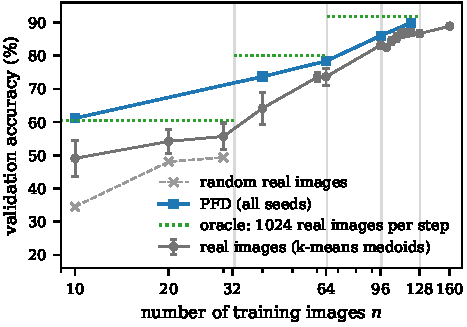
\includegraphics[width=\columnwidth]{figures/frontier.pdf}
\caption{Validation accuracy against the number of images. Real images: random draws (3 draws) and k-means medoids
(mean and standard deviation over 6 seeds, our GPU copy). PFD: sets built for all seeds (our copy, mean of 3 seeds;
at $n=120$ the scale-free set with the official script on 6 seeds). Oracle: each training step computed on 1024 real
images (seed 42). Vertical lines mark where the number of steps changes.}
\label{fig:frontier}
\end{figure}

Fig.~\ref{fig:frontier} shows how accuracy grows with $n$. Medoids are much better than random images at small $n$
(49\% against 34\% with one image per class). Accuracy then follows the steps. It jumps when a new batch, and with
it five new steps, comes in, and it drops when that batch is very small: a set of 100 medoids (a last batch of 4) is worse than a set of 96
(82.5\% against 83.2\%). Among real-image sets the score is best between 112 and 120 images (0.692 to 0.695),
where four batches give 20 steps and the last batch still holds 16 to 24 images. Beyond 128 images, more steps no
longer pay for the larger set. Our first submission was the set of 120 medoids, 12 per class (official validation
86.5\%, Kaggle score 0.692).

\subsection{PFD with 120 images}

\begin{table}[t]
\centering
\caption{Sets of 120 images. Official validation accuracy (\%) of the unmodified script on seeds 42, 0, 1, 2, 3, 4.}
\label{tab:n120}
\footnotesize
\setlength{\tabcolsep}{2.2pt}
\begin{tabular}{lccccccc}
\toprule
Set & 42 & 0 & 1 & 2 & 3 & 4 & mean\,$\pm$\,std \\
\midrule
k-means medoids & 86.49 & 87.80 & 87.48 & 88.44 & 85.78 & 87.16 & 87.19\,$\pm$\,0.95 \\
PFD, cross-entropy & 88.37 & 89.90 & 89.16 & 90.10 & 88.42 & 89.65 & 89.27\,$\pm$\,0.70 \\
PFD, scale-free & 88.40 & 90.69 & 89.65 & 91.16 & 89.51 & 90.22 & \textbf{89.94}\,$\pm$\,0.98 \\
\bottomrule
\end{tabular}
\end{table}

\begin{figure}[t]
\centering
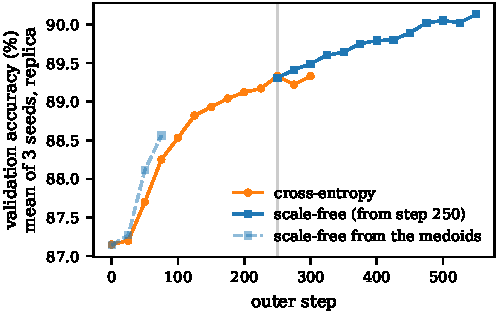
\includegraphics[width=\columnwidth]{figures/curves_n120.pdf}
\caption{Optimization at $n=120$ (validation accuracy of our GPU copy, mean of seeds 42, 0, 1). The cross-entropy run
stops improving near 89.3\%. Switching to the scale-free loss at step 250 gives steady progress. Started from the
medoids, the scale-free loss is also faster than cross-entropy.}
\label{fig:curves}
\end{figure}

Starting from the 120 medoids, PFD with the cross-entropy loss improves the official accuracy on all six seeds, by
2.08 points on average (Table~\ref{tab:n120}). The run takes about 1 h 40 min (300 outer steps, two heads per step)
and stops improving after about 250 steps (Fig.~\ref{fig:curves}). From that point, every pixel step we tried made
things worse on held-out runs, including steps computed with eight heads (Section~\ref{sec:negative}). It is a real
local optimum of the cross-entropy objective.

The scale-free loss (\ref{eq:scalefree}) moves the set out of it. Continuing from the cross-entropy optimum, it
raises the official mean to 89.94\%, and again the gain is positive on all six seeds (from $+0.03$ on seed 42 to
$+1.09$ on seed 3). Started from the medoids, it also improves faster than cross-entropy (88.56\% against 88.25\%
after 75 steps). Models trained on these sets are as accurate on 4\,050 training images as on the validation
images (89.75\% against 90.12\% for the scale-free set), so the outer loss does not overfit the real images it sees.

\begin{figure*}[t]
\centering
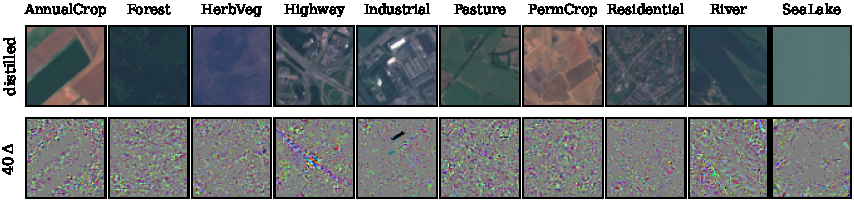
\includegraphics[width=\textwidth]{figures/images_n120.pdf}
\caption{One image per class from the 120-image scale-free set (top) and its difference with the starting medoid,
multiplied by 40 (bottom, gray means no change). The mean change is 0.26 gray levels and 78\% of the pixel values
do not change at all.}
\label{fig:images120}
\end{figure*}

The distilled images look exactly like the medoids (Fig.~\ref{fig:images120}). On average a pixel value changes by
0.26 gray levels (out of 255), 99\% of the values change by at most 2 levels, and 78\% do not change at all. These changes are too small to see, but they change the signs of many early
weight updates, and the gain holds on every seed.

\subsection{Agreement with the official script}
\label{sec:fidelity}
All our choices rely on the GPU copy, so we checked it against the official script. Over the same six seeds, the
copy gives 89.33\% for the cross-entropy set (official: 89.27\%) and 90.01\% for the scale-free set (official:
89.94\%). The official script resizes with PIL on 8-bit images, which rounds the result twice; our copy works in
float, a difference of 0.28 gray levels on average, as large as our changes. Emulating the rounding changes the mean
by 0.05 point only (89.39\% and 90.06\%). Seed by seed the two can differ by up to one point, because the two loaders
do not draw the same crops and batches. Smaller last batches make this worse. For a set of 112 images (last batch of
16), our copy gives 89.99\% over six seeds and the official script 89.24\%. Three seeds are not enough to compare two
sets: choosing the best of about 20 checkpoints on three seeds overestimated the six-seed official mean by 0.2 to 0.4
points.

\subsection{Further variants at $n=120$}

\begin{table}[t]
\centering
\caption{Variants at and near $n=120$. ``Official'' is the mean of the official script on 6 seeds; ``copy'' is our
GPU copy on the same 6 seed values. Score uses (\ref{eq:score}) with the mean accuracy.}
\label{tab:variants}
\setlength{\tabcolsep}{4pt}
\begin{tabular}{lccc}
\toprule
Variant & $n$ & accuracy (\%) & score \\
\midrule
PFD, scale-free (reference) & 120 & 89.94 official & 0.7066 \\
\quad + 150 steps with 4 heads & 120 & 90.13 copy (ref.\ 90.01) & -- \\
\quad + float32/TF32 inner training & 120 & 90.03 copy (ref.\ 90.01) & -- \\
\quad + fixed temperature $T=0.1$ & 120 & 90.00 official & 0.7069 \\
second k-means start (km1) & 120 & 89.81 copy & -- \\
best classes of two sets mixed & 120 & 89.95 copy (ref.\ 90.16) & -- \\
PFD, scale-free & 112 & 89.24 official & 0.7066 \\
\bottomrule
\end{tabular}
\end{table}

Table~\ref{tab:variants} lists what we tried on top of the scale-free set. None of it moved the six-seed mean by more
than 0.15 point. More heads per step, a more precise inner training and a lower fixed temperature all stay within
the noise of six seeds. A second start (another k-means seed) reaches the same level. Mixing the two sets class by
class, each class taken from the set where it was more accurate, was worse than either set: the classes interact
through the shared backbone updates. With 112 images the scale-free set reaches the same score as with 120, but with
a larger spread over seeds ($\pm1.34$). We kept 120.

\subsection{What did not help}
\label{sec:negative}

\begin{figure}[t]
\centering
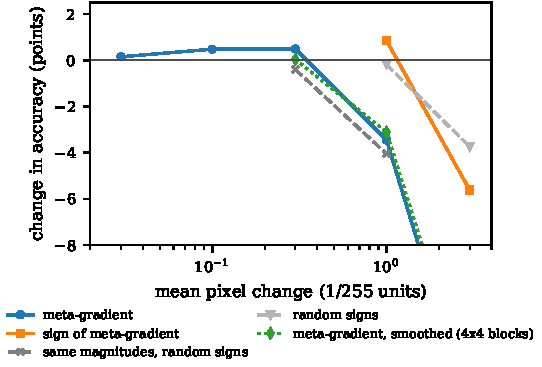
\includegraphics[width=\columnwidth]{figures/step_size.pdf}
\caption{Change in accuracy after one pixel step from the 120 medoids, measured on four held-out runs (2048 validation
images, after 8-bit rounding). The step direction comes from a meta-gradient averaged over two heads (four for the
smoothed step); its size is the mean pixel change.}
\label{fig:steps}
\end{figure}

\emph{Larger or smoother pixel steps.} From the medoids we took one step along the meta-gradient and measured the
accuracy on four other runs (Fig.~\ref{fig:steps}). Steps of 0.1 to 0.3 gray levels help ($+0.5$ point), and moving
every pixel by one level in the sign of the meta-gradient helps more ($+0.85$). One level along the plain gradient
costs 3.5 points, because the step concentrates on a few pixels with large gradients; the same magnitudes with random
signs cost 4 points. Smooth steps (the gradient averaged over $4\times4$ blocks and upsampled) are no better. The
useful information is in the fine pattern of signs. Adam directly on the pixels was four times faster at first but
stopped at 89.1\%. Averaging the gradient over random pixel noise did not help either. At the optimum, no step size and
no smoothing of the backward pass ($\tau$ from 0.03 to 3) gave a descent direction.

\emph{Other sets.} Sets of $2\times2$ mosaics of real images at half resolution, which put four images into each
training image as in~\cite{sun2024rded}, failed clearly (75.5\% at $n=120$ against 87.1\% for medoids), because the
test images are seen at full scale. Giving more images to the hardest classes (River and Highway) made the medoids
worse (86.1--86.7\% against 87.0\%). A set of 97 images, whose last batch of one adds five steps, started from 73.6\%
and reached only 77.1\%. Scaling the found pixel changes by 1.5 helped on seed 42 but not on average (89.12\%
against 89.27\%).

\subsection{Fitting the evaluation run}
\label{sec:seed42}

\begin{figure*}[t]
\centering
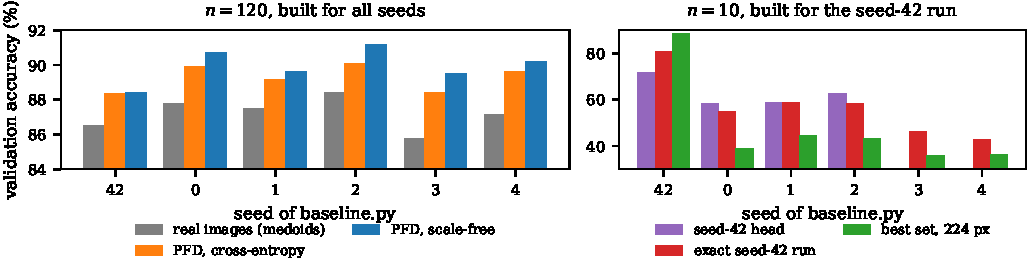
\includegraphics[width=\textwidth]{figures/per_seed.pdf}
\caption{Official validation accuracy for each seed of \texttt{baseline.py}. Left: sets of 120 images built for all
seeds. Right: sets of 10 images fitted to the seed-42 run, either to its head only or to the whole recorded run.}
\label{fig:perseed}
\end{figure*}

\begin{figure*}[t]
\centering
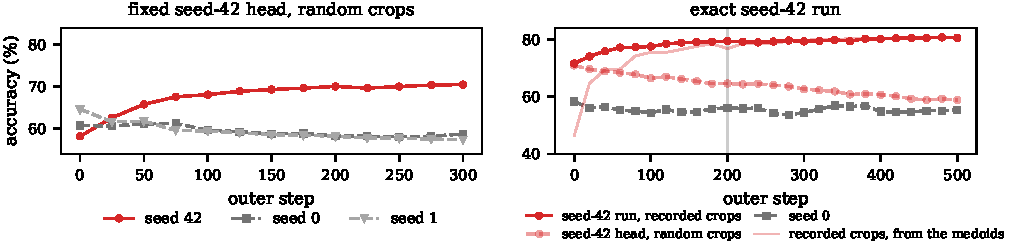
\includegraphics[width=\textwidth]{figures/seed42.pdf}
\caption{Fitting ten images to the seed-42 run. Left: the seed-42 head is fixed, crops are random; seed 42 improves
and the other seeds get worse. Right: the batches, crops and flips of the official run are recorded and replayed
(steps 0--200, then 300 more steps with a smaller step size). The faint line starts again from the medoids.}
\label{fig:seed42}
\end{figure*}

On 15 October 2026, two other teams reached scores of 0.741 and 0.731. With 120 images this
would need about 97\% accuracy, more than the oracle. These scores must come from much smaller sets that are very
accurate on the evaluation run. With one image per class, our best set built for all seeds reaches 61.2\% (score about
0.69): PFD with random heads gains 11.7 points over the medoids and passes the oracle (60.4\%), but this is far from
the 72\% needed for 0.745.

The evaluation run, however, is fixed. We first kept the seed-42 head and left the crops random (Fig.~\ref{fig:seed42},
left). In 300 steps the accuracy on seed 42 rose from 58.2\% to 70.5\%, while seeds 0 and 1 fell from 60.7\% and 64.6\%
to about 58\%. The official script confirmed it: 71.6\% on seed 42, 58.2--62.8\% on seeds 0 to 2. We then recorded the whole
run (Section~\ref{sec:method42}). Replayed in our copy with the same rounding and in float32, it matches the official
per-epoch accuracies within 0.3 point (21.4, 44.2, 64.2, 70.2 and 71.5\% against 21.4, 44.1, 64.2, 69.9 and 71.6\%).
Optimizing on it raised the seed-42 accuracy to 79.4\% in 200 steps and to 80.6\% after 280 more (official script:
80.62\%, Kaggle score 0.785, first place). On seeds 0 to 4 the same ten images give 54.8, 58.8, 58.4, 46.4 and 42.9\%
(Fig.~\ref{fig:perseed}). A run started again from the medoids reached 80.4\%, so the result does not depend on one
lucky start.

\begin{figure*}[t]
\centering
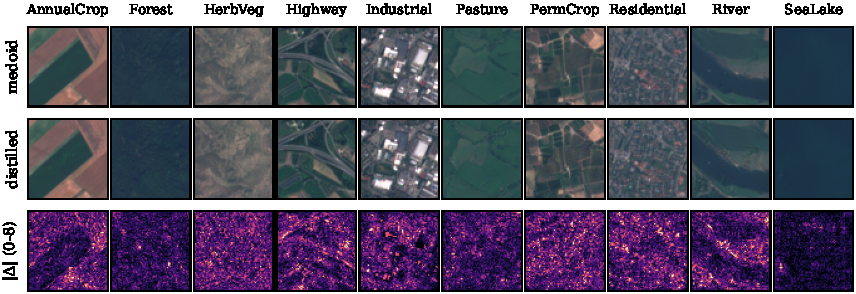
\includegraphics[width=\textwidth]{figures/images_n10.pdf}
\caption{The ten medoids (top), the set fitted to the seed-42 run (middle) and their absolute difference, averaged
over the color channels and shown from 0 to 8 gray levels (bottom). The mean change is 1.8 gray levels.}
\label{fig:images10}
\end{figure*}

These ten images still look like the medoids (Fig.~\ref{fig:images10}). The changes are larger than at $n=120$ (1.8
levels on average, at most 25, 77\% of the values changed) but remain hard to see. The set is not fragile to small
numerical differences. Turning TF32 on or off for matrix products and convolutions, which changes the rounding of
almost every operation, moved its accuracy by less than 0.1 point. It does depend on the exact draws. With random crops
and the seed-42 head it falls to 59\%, and with another seed to about 52\%. The results are exact for the run that
\texttt{baseline.py} makes with its default arguments, and only for that run.

\begin{table}[t]
\centering
\caption{Our Kaggle submissions. Validation: official script, seed 42. ``Other seeds'': mean of the official script
on other seeds (number of seeds in brackets).}
\label{tab:submissions}
\setlength{\tabcolsep}{3pt}
\begin{tabular}{rlccc}
\toprule
$n$ & Set & val.\ (42) & other seeds & Kaggle \\
\midrule
120 & k-means medoids & 86.49 & 87.33 (5) & 0.6917 \\
120 & PFD, cross-entropy & 88.37 & 89.45 (5) & 0.7026 \\
120 & PFD, scale-free & 88.40 & 90.25 (5) & 0.7034 \\
10 & PFD, seed-42 head & 71.60 & 59.91 (3) & 0.7426 \\
10 & PFD, recorded seed-42 run & 79.38 & -- & 0.7814 \\
10 & \quad + 280 more steps & 80.62 & 52.24 (5) & \textbf{0.7853} \\
\bottomrule
\end{tabular}
\end{table}

Table~\ref{tab:submissions} lists all our submissions. The difference between the two groups is large. The 120-image
sets score the same on every seed: their seed-42 result is even below their mean. The 10-image sets are 12 and 28
points better on seed 42 than on the other seeds, because the evaluation reuses the run they were fitted to.

\section{Discussion}

\emph{Why do tiny changes help?} In few-step training, the images decide the signs of the updates of 86 million
weights. Many of these weights have gradients close to zero, and a small change of the images can flip their signs.
PFD looks for changes that flip them in a useful way on average over heads and crops. This is the training-time
counterpart of an adversarial example: invisible, specific to the model and the training procedure, and helpful.
It also explains why larger steps hurt. Once a step flips many signs at random, the gain is lost.

\emph{Evaluation of distilled data.} A training set can be fitted to a single training run: its initialization, its
batch order and its augmentations. In our case it was worth about 19 points over our best 10-image set built for all seeds
(80.6\% against 61.2\%), and it moved our score from 0.703 to 0.785. Challenges and benchmarks that train once with a fixed seed reward this, whether or not it is
intended. A simple remedy is to train several times with seeds chosen at evaluation time and to score the mean. The
spread over seeds is itself useful. It was about one point for our 120-image sets and above ten points for the sets
fitted to one run. If a single run must be used, its seed and loader settings should stay hidden.

\emph{Limits.} We studied one dataset, one model and one training recipe. Our sets are made for that recipe, and we
did not test them with other optimizers, learning rates or architectures. The distillation is costly: three to four GPU
hours for a 120-image set, with 21~GB of CPU memory for the stored states. It is also not exactly repeatable, because
the GPU kernels are not deterministic. For this reason we release the exact images rather than only the code. Finally,
our numbers come from the validation set and from the public leaderboard of a challenge that was still running when
we wrote this.

\section{Conclusion}
When the model and a short fine-tuning recipe are fixed, the best training images are not the most typical ones.
They are real images with small changes that steer the few sign-like updates in a good direction. Following the
official protocol exactly, back-propagating through all its steps, and using a loss that ignores the scale of the
logits gave 120-image sets that beat the medoids on every seed by 2.7 points on average. The same tools also show
that a training set can be fitted to the evaluation run itself, which matters for anyone who evaluates distilled
data with a single training run.

\bibliographystyle{IEEEtran}
\bibliography{refs}

\end{document}
